\chapter{Integrated Vision System} \label{system}

This chapter presents an integrated vision system for the \RD{} robotics research and development platform.
The proposed system introduces new representations for images and cameras in the \RD{} environment with 
designs that prove to be modular and flexible. In this system, not only images can vary in size, pixel depth, 
and color model, but they can be easily manipulated both within and outside \RD{} through applications with 
access to the native system memory.

Moreover, this system presents a core structure for a camera that can be replicated into different camera
types, including, as shown in this chapter, a color camera and a 3D time-of-flight camera. These
representations are flexible enough to allow a camera be either a device directly connected to the computer 
running \RD{}, or a device connected remotely that transfers the image data through the network.

Section \ref{imagebuffer} of this chapter discusses the image representation in the integrated vision system, 
while Sections \ref{camera} and \ref{camerareceiver} discuss the base camera representation. 
Sections \ref{colorcam} and \ref{swissrangercam} show the flexibility of the system by presenting the 
implementations for two types of cameras. Finally, the last three sections of the chapter, Sections 
\ref{calibrationtool}, \ref{imagestream}, and \ref{packetorganizer}, further discuss some of the entities used in
the cameras' implementations.

\section{Image Buffer} \label{imagebuffer}
The \ImageBuffer{} class represents an image in the \RD{} environment. An instance of this class is defined 
by four fields. The first three are the image's width, height, and pixel depth. The fourth field can be either
the image's color model or its number of channels.\footnote{Not all images require a color model. An 
example is the depth image acquired by a range sensor.} 
The different possible combinations of values for these fields allow a flexible description of an image inside
the programming environment. Tables \ref{imagebufferdepth} and \ref{imagebuffercolormodel} show the 
available values for the depth and color model fields, as described by the \ImageBufferDepth{} and 
\ImageBufferColorModel{} enum types.

\begin{table}[ht]
\caption{Pixel depth values in the \ImageBufferDepth{} enum}
\begin{center}
\begin{tabular}{| l | l |}
	\multicolumn{2}{c}{\ImageBufferDepth{}} \\
	\hline 
	Depth 			& Description \\
	\hline \hline
	\texttt{BYTE} 		& Unsigned 8-bit integer \\
	\texttt{SHORT}	 	& Unsigned 16-bit integer \\
	\texttt{FLOAT}	 	& 32-bit floating-point single precision \\
	\texttt{DOUBLE} 	& 64-bit floating-point double-precision \\
	\hline
\end{tabular}
\end{center}
\label{imagebufferdepth}
\end{table}

\begin{table}[ht]
\caption{Color model values in the \ImageBufferColorModel{} enum}
\begin{center}
\begin{tabular}{| l | l |}
	\multicolumn{2}{c}{\ImageBufferColorModel{}} \\
	\hline 
	Color Model 		& Description \\
	\hline \hline
	\texttt{BGR} 		& Blue-Green-Red channels \\
	\texttt{BGRA} 		& Blue-Green-Red-Alpha channels \\
	\texttt{RGB}	 	& Red-Green-Blue channels \\
	\texttt{RGBA}	 	& Red-Green-Blue-Alpha channels \\
	\texttt{GRAY}	 	& Grayscale channel \\
	\hline
\end{tabular}
\end{center}
\label{imagebuffercolormodel}
\end{table}

In an image buffer, the image data is stored in an underlying \ByteBuffer{} object. 
Part of the flexibility of the \ImageBuffer{} class is attributed to the versatility of a byte buffer with
respect to the data it can hold. Furthermore, the byte buffer within an image buffer is created to be 
direct. A direct byte buffer in Java allocates its space in native system memory, outside of the Java 
virtual machine's memory heap. This allows other programs outside Java to use native code to access
the same allocated memory space. An example of the advantage of using direct buffers is the 
implementation of an interface between \RD{} and the OpenCV computer vision open source library.
This interface enables performing OpenCV functions directly onto the Java images through native code.

Pixels in an image buffer are stored row by row with interleaved channels, starting at the top-left pixel. 
The methods to access and manipulate the image data are specific to the image's pixel depth. For 
example, the methods of the form \texttt{get\-Byte\-Pix\-el} are used to access pixels in an image of depth 
\texttt{BYTE}. The different versions of the same getter method trade off convenience for performance. 
Getter methods that accept an array as input speed up a loop through the image's pixels by
avoiding the overhead of creating the output array on every call.


\section{Camera} \label{camera}
The \Camera{} abstract class is the base representation of a camera in the \RD{} environment.  As listed in 
Table \ref{cameramethods}, this class defines methods to access information about a camera 
(\texttt{get\-Width}, \texttt{get\-Height}, \texttt{get\-Time\-stamp}, \texttt{get\-Frame\-Rate}), methods to capture 
images from the camera (\texttt{start\-Cap\-turing}, \texttt{grab\-Im\-age}), and methods to perform camera 
calibration (\texttt{start\-Cal\-i\-bra\-tion}). 

\begin{table}[ht]
\caption{Public methods in the \Camera{} class}
\begin{center}
\begin{tabular}{| l |}
	\hline 
	\multicolumn{1}{| c |}{\Camera{}} \\
	\hline \hline
	\texttt{startCapturing} \\
	\texttt{startCalibration} \\
	\texttt{grabImage}	\\
	\texttt{getWidth} \\
	\texttt{getHeight} \\
	\texttt{getTimestamp} \\
	\texttt{getFrameRate} \\
	\hline
\end{tabular}
\end{center}
\label{cameramethods}
\end{table}

By providing an abstract implementation, the \Camera{} class lets its subclasses describe different types of 
cameras while specifying a common structure for them.  In this framework, \ColorCam{} and 
\SwissRangerCam{} are the main examples of extending the \Camera{} class to represent 
cameras that capture different types of data: the first one represents a conventional color camera while 
the second one represents a 3D time-of-flight camera (see Sections \ref{colorcam} and \ref{swissrangercam}). 
This design allows a flexible definition of what a camera is and lets the user choose the representation 
of the data captured by a specific sensor.

Furthermore, an object of type \Camera{} is a subtype of \DataProvider{}. A data provider is an object that 
can publish user defined datatypes in \RD{}'s  intra-application communication system, allowing other objects 
called data handlers to subscribe to and receive the provided data. In the case of a \Camera{} object, 
the provided data is represented by the abstract class \CameraData{}. Subclasses of \CameraData{}
define the datatypes captured by different camera sensors. For example, \ColorCamData{} and 
\SwissRangerCamData{} represent the data provided by \ColorCam{} and \SwissRangerCam{}, respectively.

\section{Camera Receiver} \label{camerareceiver}
The \CameraReceiver{} abstract class defines the base structure of the mechanism that will acquire and handle
data from the camera sensors. It implements two \RD{} interfaces. The first one is the \iUpdateable{} interface,
which describes classes that have an \texttt{up\-date} method. The main loop of an \RD{} application calls 
\texttt{up\-date} on all the objects that have been registered as updatable. For the camera receiver this means 
that the \texttt{up\-date} method can be used to grab an image from a camera on every loop.

The second interface used by the \CameraReceiver{} class is the \iDataRecordHandler{}. This interface is part
of \RD{}'s intra-application communication system. It is used to define a class that can handle \iDataRecord{} 
objects being sent from another application. A class that implements this interface has a 
\texttt{han\-dle\-Da\-ta\-Re\-cord} method that handles the incoming data record objects. The camera receiver
can use this method to receive records containing image data.

Table \ref{camerareceivermethods} lists the two abstract methods declared in the \CameraReceiver{} class.
These methods are used to start the image receiving process and query the receiver if it has image data 
available to be accessed or retrieved. 

\begin{table}[ht]
\caption{Public methods in the \CameraReceiver{} class }
\begin{center}
\begin{tabular}{| l |}
	\hline 
	\multicolumn{1}{| c |}{\CameraReceiver{}} \\
	\hline \hline
	\texttt{startReceiving} \\
	\texttt{isDataAvailable} \\
	\hline
\end{tabular}
\end{center}
\label{camerareceivermethods}
\end{table}
	
\section{Color Camera} \label{colorcam}
The \ColorCam{} class extends \Camera{} to represent a color camera. In the \RD{} environment, a color
camera can be a camera sensor connected directly to the computer running the system, or a camera sensor
connected to some other device that sends the images over the network to \RD{}. This versatility is provided 
by \ColorCam{} through the \ColorReceiver{} class. While the color receiver is in charge of acquiring and 
handling the images from the camera, a color camera provides access to the image buffer, the image view, 
and the camera calibration tool. Additionally, it provides the implementation of all abstract methods defined 
by the \Camera{} class. Table \ref{colorcammethods} lists the methods that a color camera adds to the 
base camera representation.

\begin{table}[ht]
\caption{Public methods in the \ColorCam{} class}
\begin{center}
\begin{tabular}{| l |}
	\hline 
	\multicolumn{1}{| c |}{\ColorCam{}} \\
	\multicolumn{1}{| c |}{{\small \texttt{extends} \Camera{}}} \\
	\hline \hline
	\texttt{getImage} \\
	\texttt{getImageView} \\
	\texttt{getCalibrationTool} \\
	\hline
\end{tabular}
\end{center}
\label{colorcammethods}
\end{table}

There are two ways of accessing the camera's images. One way is through the \ColorCam{} object's internal 
image buffer, which stores a copy of the last grabbed image. This image buffer is obtained by calling the
\texttt{get\-Im\-age} method. The second way takes advantage of \RD{}'s intra-application communication 
system and consists of subscribing to the data objects of type \ColorCamData{} through the \DataHandler{} 
interface. The \texttt{han\-dle\-Da\-ta} method of the data handler receives the data objects that contain an 
image buffer with the copy of the grabbed image.

Therefore, every time a call to \texttt{grab\-Im\-age} returns successfully (i.e. returns a \texttt{true} value) two 
things happen: (1) the acquired image is stored in the internal image buffer and (2) it is published through the 
\DataProvider{} interface. Accessing the images from the image buffer gives the user more precision when it
is necessary to process the image right after it is grabbed. Receiving a published image contains the 
overhead of going through the data dispatcher mechanism, but simplifies the communication between
\RD{} applications. 

The \ColorCam{} class adds a second version of the \texttt{grab\-Im\-age} method. This second version takes
as input a value that represents the desired timestamp for the grabbed image. This method is 
useful when synchronizing two or more cameras: given the timestamp of an image from one of the cameras
this \texttt{grab\-Im\-age} method can be used to retrieve the closest corresponding image from the other
cameras.  

A color camera also provides the option of displaying the image stream using \RD{}'s graphics display system.
This is achieved by instantiating an \ImageView{} object linked to the color camera's internal image buffer. 
Every time an image is acquired the image view needs to be refreshed in order to display the new data on the 
buffer. This image view is accessed by calling the \texttt{get\-Im\-age\-View} method.

Finally, the methods to perform camera calibration and retrieve the camera's parameters are available 
through the \CalibrationTool{} object that is associated with every instance of \ColorCam{}. Upon the creation
of the color camera, a calibration tool object is constructed and linked to the camera's internal image buffer. 
When the \texttt{start\-Cal\-i\-bra\-tion} method is called, the calibration tool is started. Then, the user can
use the methods in the calibration tool, obtained by calling the \texttt{get\-Cal\-i\-bra\-tion\-Tool} method, to 
calibrate the camera (see Section \ref{calibrationtool}). 

The following sections present and discuss the modules that compose the \ColorCam{} class. The 
module dependency diagram in Figure \ref{colorcammoduledependency} shows how these classes 
are related to each other. 

\begin{figure}[t]
\begin{center}
\digraph[scale=0.75]{ColorCam}{
	graph [rankdir = "TB" margin = 0];
	node [shape = "box" style = "filled" fillcolor = "gainsboro" fontsize = "12" fontname = "Courier"];
		Camera CameraReceiver CameraData Stream;
	node [shape = "box" style = "filled" fillcolor = "floralwhite" fontsize = "12" fontname = "Courier"];
	{ rank = "source"; CameraReceiver Camera CameraData Stream;}
	{ rank = "same"; ColorCam ColorCamData;}
	{ rank = "same"; ColorReceiver CalibrationTool;}
	{ rank = "same"; ColorPacketHandler DC1394JavaAcquire ImageStream;}
	{ rank = "sink"; PacketOrganizer;}
	edge [arrowhead = "normal"];
	Camera -> CameraData;
	ColorCam -> Camera [arrowhead = "empty"] ;
	ColorCam -> ColorCamData;
	ColorCam -> ColorReceiver ;
	ColorCam -> CalibrationTool;
	ColorCamData -> CameraData [arrowhead = "empty"];
	ColorReceiver -> CameraReceiver [arrowhead = "empty"];
	ColorReceiver -> ColorPacketHandler;
	ColorReceiver -> DC1394JavaAcquire;
	ColorReceiver -> ImageStream;
	ImageStream -> Stream [arrowhead = "empty"];
	ColorPacketHandler -> PacketOrganizer;
}
\caption[\ColorCam{}'s module dependency diagram]{\ColorCam{} module dependency diagram. Arcs with 
white arrows represent subtype relations (A $\vartriangleright$ B = A extends B) while arcs with black arrows 
represent implementation relations (A $\blacktriangleright$ B = A uses B). Gray rectangles represent abstract 
classes. The \ImageBuffer{} class is omitted from this diagram.}
\label{colorcammoduledependency}
\end{center}
\end{figure}



	
	\subsection{Color Receiver} \label{colorreceiver}
	The \ColorReceiver{} class extends \CameraReceiver{} to provide the mechanism that interfaces with a color 
camera. It allows the user to acquire images directly from a Firewire camera or to receive the color images via a 
network transfer. Image acquisition from the camera is achieved using the libdc1394 API, a library of functions to 
control Firewire cameras that conform to the 1394-based Digital Camera Specifications \cite{libdc1394}. The 
network transfer is achieved through IRCP, the network communication protocol used by \RD{} \cite{IRCP}.
Table \ref{colorreceivermethods} lists the methods that the \ColorReceiver{} class adds to the camera receiver 
representation.

\begin{table}[ht]
\caption{Public methods in the \ColorReceiver{} class }
\begin{center}
\begin{tabular}{| l |}
	\hline 
	\multicolumn{1}{| c |}{\ColorReceiver{}} \\
	\multicolumn{1}{| c |}{{\small \texttt{extends} \CameraReceiver{}}} \\
	\hline \hline
	\texttt{getImage} \\
	\texttt{handleDataRecord} \\
	\texttt{update} \\
	\hline
\end{tabular}
\end{center}
\label{colorreceivermethods}
\end{table}

Upon initialization, the color receiver first tries to connect to a Firewire camera. The \texttt{up\-date} method
is in charge of acquiring the images using the \DCJavaAcquire{} methods. If the color receiver does not find a 
camera or if it fails when attempting to connect to one, it will proceed to start the IRCP network connection by 
setting up a \ColorPacketHandler{} (the user has the option of forcing this network connection). As discussed in 
Section \ref{camerareceiver}, the images received by the packet handler are sent to the color receiver through 
the \iDataRecordHandler{} interface. The color receiver calls the \texttt{han\-dle\-Da\-ta\-Re\-cord} method to 
handle the incoming data record objects.

The \ColorReceiver{} class is flexible with the type of image it can handle. The image type is specified by a 
set of public static variables that the user can modify. Table \ref{colorreceivervariables} contains the list of all 
the variables available to the user. When running on libdc1394 mode the user can change the size of the image 
captured from the camera. When running on network mode the user can modify the image size, pixel depth, and 
color model according to what is being transferred over the network. 

\begin{table}[ht]
\caption{User-modifiable static variables in the \ColorReceiver{} class}
\begin{center}
\begin{tabular}{| l | l |}
	\multicolumn{2}{c}{\ColorReceiver{}} \\
	\hline
	Variable & Description \\
	\hline \hline
	\texttt{WIDTH} 						& The image width \\
	\texttt{HEIGHT} 					& The image height \\
	\texttt{DEPTH} 						& The image pixel depth \\
	\texttt{COLOR\_MODEL} 				& The image color model \\
	\texttt{CAMERA\_GUID} 				& The camera GUID \\
	\texttt{DC1394\_FRAME\_RATE} 		& The camera capturing frame rate \\
	\texttt{DC1394\_ISO\_SPEED} 			& The camera ISO speed \\
	\texttt{UNDISTORT} 				& Flag to undistort the image \\
	\texttt{COMPRESSED\_IMAGE} 		& Flag if image is compressed \\
	\texttt{STREAM\_CAPACITY} 			& The receiver image stream size \\
	\texttt{VISION\_MINOR\_TYPE} 		& The IRCP minor type \\
	\texttt{PACKET\_HANDLER\_NAME} 	& The packet handler name \\
	\texttt{PACKET\_HANDLER\_KEY} 				& The packet handler key \\
	\hline
\end{tabular}
\end{center}
\label{colorreceivervariables}
\end{table}

Besides handling a real time image stream, the color receiver can store a user-defined number of last seen 
images in memory. The mechanism that processes the image stream works like a First-In-First-Out queue: 
fresh images are stored at the tail of the stream while old images are retrieved from the head of the stream. 
The size of the stream determines the number of images that can be saved in memory. This system allows
to synchronize two or more cameras by finding in their streams the images with matching (or closest) 
timestamp. The \ImageStream{} class contains the implementation of this mechanism (see Section 
\ref{imagestream}).

	\subsection{Color Packet Handler} \label{colorpackethandler}
	The \ColorPacketHandler{} class is a subtype of \SafePacketHandler{}, a class part of the receiving end in 
the IRCP communication system. The \ColorReceiver{} object creates a color packet handler to manage the 
packets sent over the network that correspond to image data from a color camera. Therefore, the color
packet handler needs to know how the color information is encoded in the incoming packet. 

In order to manage a large number of sent packets, some of which can get lost or arrive out of sequence, 
the color packet handler implementation uses a \PacketOrganizer{} object to organize the incoming 
data (see Section \ref{packetorganizer}). The packet organizer takes the received packets, which 
consist of subparts of the whole image, and informs the color packet handler once there are images ready
to be retrieved.

Table \ref{colorpackethandlermethods} contains the method that the color packet handler overrides 
from the safe packet handler class. 

\begin{table}[ht]
\caption{Public methods in the \ColorPacketHandler{}  class}
\begin{center}
\begin{tabular}{| l |}
	\hline 
	\multicolumn{1}{| c |}{\ColorPacketHandler{}} \\
	\multicolumn{1}{| c |}{{\small extends \SafePacketHandler{}}} \\
	\hline \hline
	\texttt{safeHandle} \\
	\hline
\end{tabular}
\end{center}
\label{colorpackethandlermethods}
\end{table}
	\subsection{DC1394 Java Acquire} \label{dc1394javaacquire}
	The \DCJavaAcquire{} class establishes the Java interface to the libdc1394 library. Since libdc1394 is 
written in C, this class uses the Java Native Interface (JNI) framework to access the library functions.
The native methods declared in the Java layer are implemented in a separate C layer, and this
implementation is packaged in the \RD{} JNI library called libdc1394\-Ja\-va\-Ac\-quire. 

The \DCJavaAcquire{} class simplifies the access to a Firewire camera by declaring the methods listed
in Table \ref{dcjavaacquiremethods}. The \texttt{get\-GUIDs} method returns a list of GUIDs from the 
available Firewire cameras, and \texttt{start\-Cap\-tur\-ing}, \texttt{stop\-Cap\-tur\-ing}, and \texttt{get\-Im\-age}
are used to control and acquire images from them. The last two methods in the list are specific to Firewire 
cameras produced by Point Grey, and they are used to convert captured grayscale images to color images.

\begin{table}[ht]
\caption{Public methods in the \DCJavaAcquire{} class}
\begin{center}
\begin{tabular}{| l |}
	\hline 
	\multicolumn{1}{| c |}{\DCJavaAcquire{}} \\
	\hline \hline
	\texttt{getGUIDs} \\
	\texttt{startCapturing} \\
	\texttt{stopCapturing} \\
	\texttt{getImage} \\
	\texttt{retrievePointGreyBayerTile} \\
	\texttt{convertPointGreyMonoToBGR} \\
	\hline
\end{tabular}
\end{center}
\label{dcjavaacquiremethods}
\end{table}
	
\section{SwissRanger Camera} \label{swissrangercam}
The \SwissRangerCam{} class and its components are very similar to the classes that describe a color 
camera in \RD{}. This proves that the system can represent cameras following a similar core structure. Like 
\ColorCam{}, the \SwissRangerCam{} class extends \Camera{}. In this case it represents a SwissRanger
sensor, a 3D time-of-flight camera produced by Mesa Imaging \cite{SR4000Manual}. The SwissRanger 
can capture depth information (z-coordinates) from a scene, as well as x-coordinates and y-coordinates for 
each of the depth points. Associated with this data is the amplitude and the confidence map, which provide
measurements of the quality of the acquired data. 

In the representation, the SwissRanger can be connected directly to the computer running the system, or it 
can be connected to some other device that sends the images over the network to \RD{}. This versatility is 
provided through the \SwissRangerReceiver{} class. While the SwissRanger receiver is in charge of acquiring 
and handling the images from the camera, the SwissRanger camera provides access to the image buffers, 
the image views, and the camera calibration tool, as well as the implementation of all abstract methods 
defined by the \Camera{} class. Furthermore, it contains the information about the modulation frequency 
on which the SwissRanger is running, and static methods to create visualizations for the depth and amplitude 
data. Table \ref{swissrangercammethods} lists the methods that the SwissRanger class adds to the base 
camera representation.

\begin{table}[ht]
\caption{Public methods in the \SwissRangerCam{} class}
\begin{center}
\begin{tabular}{| l |}
	\hline 
	\multicolumn{1}{| c |}{\SwissRangerCam{}} \\
	\multicolumn{1}{| c |}{{\small \texttt{extends} \Camera{}}} \\
	\hline \hline
	\texttt{getDepth} \\
	\texttt{getAmplitude} \\
	\texttt{getX} \\
	\texttt{getY} \\
	\texttt{getConfidenceMap} \\
	\texttt{getDepthDisplay} \\
	\texttt{getAmplitudeDisplay} \\
	\texttt{getDepthView} \\
	\texttt{getAmplitudeView} \\
	\texttt{getCalibrationTool} \\
	\texttt{getModulationFrequency} \\
	\texttt{createDisplays} \\
	\texttt{threshold} \\
	\texttt{toMeters} \\
	\hline
\end{tabular}
\end{center}
\label{swissrangercammethods}
\end{table}

There are two ways of accessing the image data captured by the SwissRanger. One way is through the 
camera object's internal image buffers, which store copies of the last grabbed images. The depth data
is obtained by calling the \texttt{get\-Depth} method, and the amplitude data is obtained by calling 
\texttt{get\-Am\-pli\-tude}. The x-coordinate, y-coordinate, and confidence map data are obtained by calling
\texttt{getX}, \texttt{getY}, and \texttt{get\-Con\-fi\-dence\-Map}, respectively.

The second way takes advantage of \RD{}'s intra-application communication system and consists of 
subscribing to the data objects of type \SwissRangerCamData{} through the \DataHandler{} interface. 
A SwissRanger data object contains the same number of image buffers as described before, each with a 
copy of the last grabbed image. The \texttt{han\-dle\-Da\-ta} method of the data handler receives these data 
objects. 

Similar to the \ColorCam{} class, when the \texttt{grab\-Im\-age} method returns successfully the acquired 
images are stored in the internal image buffers and then are published through the \DataProvider{} interface. 
Accessing the images directly from the image buffers avoids the overhead of going through the data 
dispatcher mechanism and allows the user to process the images right after they are grabbed. However, 
receiving the images published through the data dispatcher simplifies the communication between \RD{} 
applications. 

Furthermore, the \SwissRangerCam{} class also adds a second version of the \texttt{grab\-Im\-age} method.
The reason for this method becomes clearer now. A Firewire color camera could be synchronized with a 
SwissRanger, but differences in the devices and their capturing mechanisms might not give the user the 
same capturing frame rate nor the same timestamp for images captured at the same time. Since this second 
version of the \texttt{grab\-Im\-age} method takes as input a desired timestamp for the grabbed image, it is 
possible to get a timestamp from one of the cameras and retrieve the closest corresponding image from the 
second camera taking into account a timestamp offset.

The \SwissRangerCam{} class provides the option of displaying visualizations for the depth image stream 
and the amplitude image stream. The methods \texttt{get\-Depth\-Dis\-play} and 
\texttt{get\-Am\-pli\-tude\-Dis\-play} return image buffers with BGR color model and \texttt{BYTE} pixel depth 
containing the image data of the visualizations. These image buffers are linked to \ImageView{} objects and 
are obtained through the \texttt{get\-Depth\-View} and \texttt{get\-Am\-pli\-tudeView} methods. The method 
\texttt{cre\-ate\-Dis\-plays} is used to create the visualizations from the raw depth and amplitude data.

The \CalibrationTool{} class is again used to provide the methods that perform camera calibration and retrieve
the camera's parameters. Since the amplitude image is visually close to a grayscale image, the calibration tool 
object is linked to the internal amplitude image buffer of the \SwissRangerCam{} instance. The user can 
access this object through the \texttt{get\-Cal\-i\-bra\-tion\-Tool} method, and then calibrate the camera by 
using the methods discussed in Section \ref{calibrationtool}.

The following sections present and discuss the modules that make up the \SwissRangerCam{} class. Figure 
\ref{swissrangercammoduledependency} shows a module dependency diagram that indicates how these 
classes are related to each other. 

\begin{figure}[t]
\begin{center}
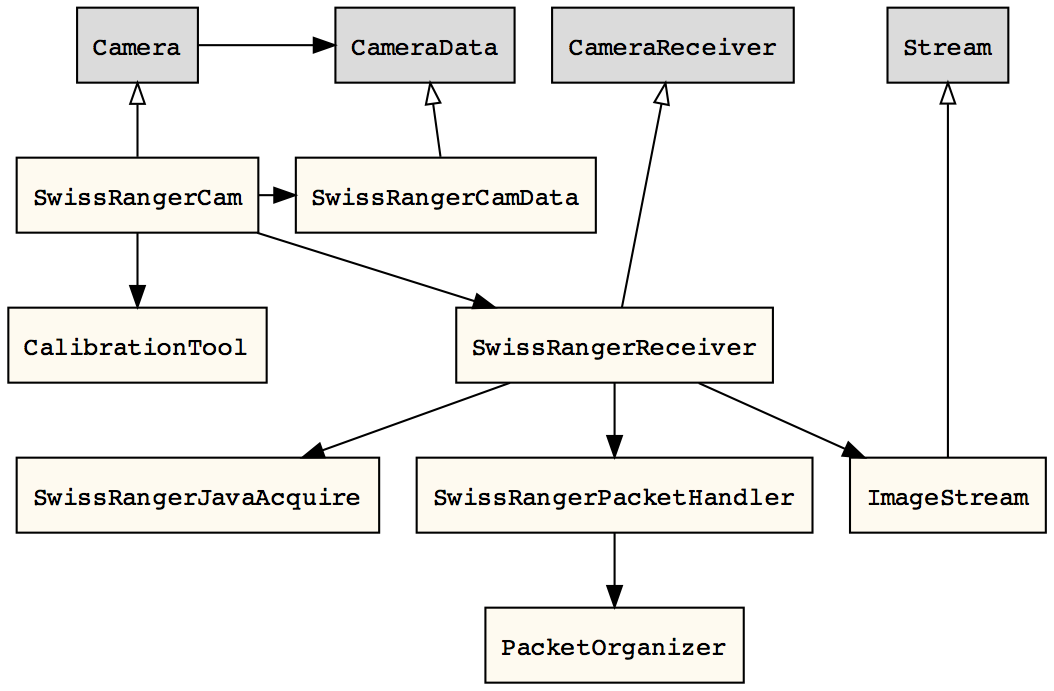
\includegraphics[width = 15cm]{SwissRangerCam.png}
%\digraph[scale=0.75]{SwissRangerCam}{
	graph [rankdir = "TB" margin = 0];
	node [shape = "box" style = "filled" fillcolor = "gainsboro" fontsize = "12" fontname = "Courier"];
		Camera CameraReceiver CameraData Stream;
	node [shape = "box" style = "filled" fillcolor = "floralwhite" fontsize = "12" fontname = "Courier"];
	{ rank = "source"; CameraReceiver Camera CameraData Stream;}
	{ rank = "same"; SwissRangerCam SwissRangerCamData;}
	{ rank = "same"; SwissRangerReceiver CalibrationTool;}
	{ rank = "same"; SwissRangerPacketHandler SwissRangerJavaAcquire ImageStream;}
	{ rank = "sink"; PacketOrganizer;}
	edge [arrowhead = "normal"];
	Camera -> CameraData;
	SwissRangerCam -> Camera [arrowhead = "empty"] ;
	SwissRangerCam -> SwissRangerCamData;
	SwissRangerCam -> SwissRangerReceiver ;
	SwissRangerCam -> CalibrationTool;
	SwissRangerCamData -> CameraData [arrowhead = "empty"];
	SwissRangerReceiver -> CameraReceiver [arrowhead = "empty"];
	SwissRangerReceiver -> SwissRangerPacketHandler;
	SwissRangerReceiver -> SwissRangerJavaAcquire;
	SwissRangerReceiver -> ImageStream;
	ImageStream -> Stream [arrowhead = "empty"];
	SwissRangerPacketHandler -> PacketOrganizer;
}
\caption[\SwissRangerCam{}'s module dependency diagram]{\SwissRangerCam{} module dependency 
diagram. Arcs with white arrows represent subtype relations (A $\vartriangleright$ B = A extends B) while 
arcs with black arrows represent implementation relations (A $\blacktriangleright$ B = A uses B). Gray 
rectangles represent abstract classes. The \ImageBuffer{} class is omitted from this diagram.}
\label{swissrangercammoduledependency}
\end{center}
\end{figure}

	
	\subsection{SwissRanger Receiver} \label{swissrangerreceiver}
	The \SwissRangerReceiver{} class extends \CameraReceiver{} to provide the mechanism that interfaces with a 
SwissRanger camera. It allows the user to acquire images directly from a SwissRanger or to receive depth, 
amplitude, x-coordinate, y-coordinate, and confidence images via a network transfer. Image acquisition from 
the camera is achieved using the SwissRanger driver API that is provided by Mesa Imaging. The network 
transfer is achieved through IRCP. Table \ref{swissrangerreceivermethods} lists the methods of the 
SwissRanger receiver class.

\begin{table}[ht]
\caption{Public methods in the \SwissRangerReceiver{} class}
\begin{center}
\begin{tabular}{| l |}
	\hline 
	\multicolumn{1}{| c |}{\SwissRangerReceiver{}} \\
	\multicolumn{1}{| c |}{{\small \texttt{extends} \CameraReceiver{}}} \\
	\hline \hline
	\texttt{getDepth} \\
	\texttt{getAmplitude} \\
	\texttt{getX} \\
	\texttt{getY} \\
	\texttt{getConfidenceMap} \\
	\texttt{handleDataRecord} \\
	\texttt{update} \\
	\hline
\end{tabular}
\end{center}
\label{swissrangerreceivermethods}
\end{table}

Similar to the color receiver, the SwissRanger receiver first tries to connect to a Swiss\-Ranger camera. The 
\texttt{up\-date} method, called on each system loop, grabs the images from the camera using the 
\SwissRangerJavaAcquire{} methods. If the receiver fails to connect to a camera it proceeds to start the IRCP 
network connection by setting up a \SwissRangerPacketHandler{} (again, the user has the option of forcing a 
network connection). The images received by the packet handler are sent to the SwissRanger receiver, which 
calls the \texttt{han\-dle\-Da\-ta\-Re\-cord} method to handle the incoming data record objects.

The \SwissRangerReceiver{} class is flexible with the type of image it can handle and it provides a set of 
public static variables that the user can modify. However, in practice these variables are not changed 
because the SwissRanger sensor itself does not provide this flexibility. Table \ref{swissrangerreceivervariables} 
contains the list of all the variables available to the user. As this table shows, the user has the option of 
thresholding the depth image. This thresholding is performed based on depth, amplitude, and confidence map
values. 

\begin{table}[ht]
\caption{User-modifiable static variables in the \SwissRangerReceiver{} class}
\begin{center}
\begin{tabular}{| l | l |}
	\multicolumn{2}{c}{\SwissRangerReceiver{}} \\
	\hline
	Variable & Description \\
	\hline \hline
	\texttt{WIDTH} 								& The image width \\
	\texttt{HEIGHT} 							& The image height \\
	\texttt{DEPTH} 								& The image pixel depth \\
	\texttt{NUMBER\_OF\_CHANNELS} 				& The image number of channels \\
	\texttt{MODULATION\_FREQUENCY} 			& The modulation frequency of the camera \\
	\texttt{INITIAL\_DEPTH\_HIGH\_THRESHOLD} 	& The initial depth high threshold \\
	\texttt{INITIAL\_DEPTH\_LOW\_THRESHOLD} 	& The initial depth low threshold \\
	\texttt{INITIAL\_AMPLITUDE\_THRESHOLD} 		& The initial amplitude threshold \\
	\texttt{INITIAL\_CONFIDENCE\_THRESHOLD} 	& The initial confidence threshold \\
	\texttt{MAX\_AMPLITUDE\_THRESHOLD} 		& The maximum threshold for the amplitude \\
	\texttt{MAX\_CONFIDENCE\_THRESHOLD} 		& The maximum threshold for the confidence \\
	\texttt{UNDISTORT} 						& Flag to undistort the image \\
	\texttt{THRESHOLD} 						& Flag to threshold the depth image \\
	\texttt{STREAM\_CAPACITY} 					& The receiver image stream size \\
	\texttt{VISION\_MINOR\_TYPE} 				& The IRCP minor type \\
	\texttt{PACKET\_HANDLER\_NAME} 			& The packet handler name \\
	\texttt{PACKET\_HANDLER\_KEY} 				& The packet handler key \\
	\hline
\end{tabular}
\end{center}
\label{swissrangerreceivervariables}
\end{table}

The Swiss\-Ranger receiver handles the different image streams using the First-In-First-Out queue mechanism 
used by the color receiver: fresh images are stored at the tail of the stream while old images are retrieved 
from the head of the stream. This allows the receiver to store a user-defined number of last seen images in 
memory and to synchronize two or more cameras by locating in their streams the images with matching (or 
closest) timestamp. Like in the \ColorReceiver{} class, the implementation of this mechanism is provided by an 
\ImageStream{} object (see Section \ref{imagestream}).

	\subsection{SwissRanger Packet Handler} \label{swissrangerpackethandler}
	The \SwissRangerPacketHandler{} class contains the information about how the Swiss\-Ranger data is encoded 
in incoming network packets. It is a subtype of \SafePacketHandler{}, and it is instantiated by the Swiss\-Ranger 
receiver in order to manage the Swiss\-Ranger image data transferred over the network.

Similar to the \ColorPacketHandler{}, this class uses a \PacketOrganizer{} in its implementation to sort and 
organize the large number of incoming packets (see Section \ref{packetorganizer}). The packet organizer puts 
together the received images' pieces and informs the SwissRanger packet handler once they are ready to be 
retrieved. Table \ref{swissrangerpackethandlermethods} lists the method that the SwissRanger packet handler 
overrides from the \SafePacketHandler{} class. 

\begin{table}[ht]
\caption{Public methods in the \SwissRangerPacketHandler{}}
\begin{center}
\begin{tabular}{| l |}
	\hline 
	\multicolumn{1}{| c |}{\SwissRangerPacketHandler{}} \\
	\multicolumn{1}{| c |}{{\small extends \SafePacketHandler{}}} \\
	\hline \hline
	\texttt{safeHandle} \\
	\hline
\end{tabular}
\end{center}
\label{swissrangerpackethandlermethods}
\end{table}
	\subsection{SwissRanger Java Acquire} \label{swissrangerjavaacquire}
	The \SwissRangerJavaAcquire{} class establishes the Java interface to the SwissRanger driver. It uses the 
Java Native Interface (JNI) framework to access the native functions in the driver's library. The \RD{} Java layer 
declares native methods that are implemented in a C layer packaged in the \RD{} JNI library called 
libsrJavaAcquire. 

The \SwissRangerJavaAcquire{} class simplifies the access to a SwissRanger camera by declaring the 
method listed in Table \ref{swissrangerjavaacquiremethods}. Unlike \DCJavaAcquire{}, this class does not
declare \texttt{start\-Cap\-tur\-ing} nor \texttt{stop\-Cap\-tur\-ing} methods. The driver's library does not contain
functions equivalent to these operations since the camera is capturing from the moment it is created.
The \texttt{getImages} method is used to retrieve the images for all data types at the same time.  

\begin{table}[ht]
\caption{Public methods in the \SwissRangerJavaAcquire{} class}
\begin{center}
\begin{tabular}{| l |}
	\hline 
	\multicolumn{1}{| c |}{\SwissRangerJavaAcquire{}} \\
	\hline \hline
	\texttt{getImages} \\
	\hline
\end{tabular}
\end{center}
\label{swissrangerjavaacquiremethods}
\end{table}

		
\section{Calibration Tool} \label{calibrationtool}
The \CalibrationTool{} class provides methods to calibrate a camera, undistort the camera images using the 
output of the calibration, and save the output into a file. A calibration tool object is created by providing the 
image buffer associated with the camera that is to be calibrated. Table \ref{calibrationtoolmethods} lists 
all methods available in the \CalibrationTool{} class.

\begin{table}[ht]
\caption{Public methods in the \CalibrationTool{} class}
\begin{center}
\begin{tabular}{| l |}
	\hline 
	\multicolumn{1}{| c |}{\CalibrationTool{}} \\
	\hline \hline
	\texttt{start} \\
	\texttt{reset} \\
	\texttt{isCalibrating} \\
	\texttt{calibrate} \\
	\texttt{findAndDrawCorners} \\
	\texttt{addCornersToList} \\
	\texttt{calibrateCamera} \\
	\texttt{initUndistortMap} \\
	\texttt{undistort} \\
	\texttt{setCameraParameters} \\
	\texttt{setChessboardDimensions} \\
	\texttt{setChessboardSquareSize} \\
	\texttt{setRequiredSamples} \\
	\texttt{setWindowDimensions} \\
	\texttt{getCameraParameters} \\
	\texttt{getCameraParametersPath} \\
	\texttt{getChessboardNumberOfColumns} \\
	\texttt{getChessboardNumberOfRows} \\
	\texttt{getChessboardSquareSize} \\
	\texttt{getRequiredSamples} \\
	\texttt{getWindowWidth} \\
	\texttt{getWindowHeight} \\
	\texttt{loadCameraParameters} \\
	\texttt{saveCameraParameters} \\ 
	\texttt{getVectorFromUndistortedCameraImage} \\
	\hline
\end{tabular}
\end{center}
\label{calibrationtoolmethods}
\end{table}

The implementation of the \CalibrationTool{} is based on the calibration functions of the OpenCV open source 
library, which in turn are based on Jean-Yves Bouguet's implementation of Zhang's calibration method
\cite{Bouguet, Zhang}. The calibration process is started by calling the \texttt{start} method, and at any
time it can be restarted by calling \texttt{re\-set} followed by \texttt{start}. The process consists of detecting a 
checkerboard pattern (Figure \ref{checkerboard}) on multiple images until acquiring a preset number of 
calibration images. The information about the position of the checkerboard's corners is extracted from the 
images and then fed to the calibration algorithm. The algorithm for one loop of the calibration process, which 
runs on each user call to the method \texttt{cal\-i\-brate}, is described in Table \ref{calibratealgorithm}.

\begin{figure}[t]
\begin{center}
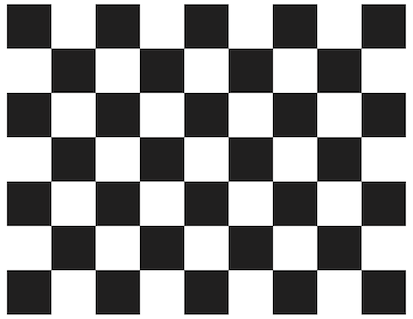
\includegraphics[scale=0.9]{checkerboard.png}
\caption{Checkerboard pattern used for camera calibration}
\label{checkerboard}
\end{center}
\end{figure}

\begin{table}[ht]
\caption{Algorithm for the \texttt{calibrate} method in \CalibrationTool{}}
\begin{center}
\begin{tabular}{ l l }
\hline
\multicolumn{2}{l}{\texttt{CALIBRATE (currentImages, requiredImages):}} \\
1 & \texttt{{\bf If} (currentImages < requiredImages)} \\
2 & \hspace{0.6cm} \texttt{\bf Then:} \\
3 & \hspace{1.2cm} \texttt{Search checkerboard pattern in the image;} \\
4 & \hspace{1.2cm} \texttt{{\bf If} the pattern is found} \\
5 & \hspace{1.8cm} \texttt{\bf Then:} \\
6 & \hspace{2.4cm} \texttt{Extract the corners and save them;} \\
7 & \hspace{2.4cm} \texttt{Increment currentImages counter;} \\
8 & \hspace{0.6cm} \texttt{\bf Else:} \\
9 & \hspace{1.2cm} \texttt{Run calibration algorithm with saved corners;} \\
\hline
\end{tabular}
\end{center}
\label{calibratealgorithm}
\end{table}

The algorithm starts by checking if the count of acquired images is less than the number of required images.
If it is, it calls the \texttt{find\-And\-Draw\-Cor\-ners} method to search the image for the position of the 
calibration pattern's corners (line 3). If the complete set of corners is found, \texttt{add\-Cor\-ners\-To\-List} is 
called in order to save their positions into a list (line 6), and then the count of acquired images is incremented
(line 7). Therefore, the user must call \texttt{cal\-i\-brate} until the number of acquired images reaches 
the number of required images. Once it reaches it, an additional call to \texttt{cal\-i\-brate} runs the camera 
calibration algorithm by calling the \texttt{cal\-i\-brate\-Cam\-er\-a} method (line 9). At any point of the 
calibration process the user can call \texttt{is\-Cal\-i\-brat\-ing} to check if the calibration tool is waiting for 
more images.

Once the camera calibration is performed, the results are saved into an object of type \CameraParameters{}
which is accessed through the \texttt{get\-Cam\-e\-ra\-Pa\-ram\-e\-ters} method. This object holds the 
intrinsic parameters (focal length, principal point, distortion coefficients) and extrinsic parameters 
(rotation and translation vectors) that describe the camera. The camera parameters can be saved into 
or read from an XML file using the \texttt{save\-Cam\-er\-aPa\-ram\-e\-ters} and 
\texttt{load\-Cam\-er\-a\-Pa\-ram\-e\-ters} methods, respectively. 

Finally, the \CalibrationTool{} class provides the methods to undistort the camera images given the camera's
parameters values. First, the x-coordinate and y-coordinate pixel undistortion maps need to be created by 
calling the \texttt{in\-it\-Un\-dis\-tort\-Map} method. This method assumes that the camera parameters object 
has been set, either by running the calibration process, loading the parameters from a file, or setting the 
object using the \texttt{set\-Cam\-er\-a\-Pa\-ram\-e\-ters} method. After initializing the undistortion maps, 
each call to the \texttt{un\-dis\-tort} method will undistort the image in the calibration tool's image buffer.



	
\section{Image Stream} \label{imagestream}

	The \ImageStream{} class is used by the \ColorReceiver{} and \SwissRangerReceiver{}  classes to 
	handle the image streams from the cameras (see Sections \ref{colorreceiver} and 
	\ref{swissrangerreceiver}). Section \ref{stream} describes the superclass of \ImageStream{}, the 
	\Stream{} abstract class. Section \ref{imagestream2} describes the \ImageStream{} class itself.

	\subsection{Stream} \label{stream}
	The \Stream{} abstract class represents a stream of buffer objects. A buffer object can be any mutable object 
used to store data. Since the \Stream{} class is defined using a generic type declaration, it allows the user
decide what will the buffer object be in an specific stream implementation. 

When deciding on a buffer object, the user has to make sure it can be created and manipulated using the 
abstract methods listed in Table \ref{streamprotectedmethods}. These methods should be implemented by 
the user in the \Stream{}'s subclasses, where \texttt{T} is substituted by the type of the buffer object. The 
\texttt{buff\-er} argument in the \texttt{write\-Buff\-er} and \texttt{read\-Buff\-er} methods represents the buffer
where data is going to be written or from where data is going to be read, respectively. Conversely, the 
\texttt{da\-ta} argument represents the data that will be written into the buffer or where the data read from the 
buffer will be copied into, respectively.

\begin{table}[ht]
\caption{Abstract methods that define the buffer object in the \Stream{} class}
\begin{center}
\begin{tabular}{| l |}
	\hline 
	\multicolumn{1}{| c |}{\Stream{}} \\
	\hline \hline
	\texttt{T createBuffer()} \\
	\texttt{writeBuffer(T buffer, T data)} \\
	\texttt{readBuffer(T buffer, T data)} \\
	\hline
\end{tabular}
\end{center}
\label{streamprotectedmethods}
\end{table}

The \Stream{} object is created with a finite capacity that remains constant during the lifetime of the object. 
Therefore, it creates a finite amount of buffer objects that are instantiated only once and always reused 
afterwards. The \Stream{} class' design allows to operate similar to a First-In-First-Out queue, with the 
incoming data being added at the tail of the stream and the old data being polled from the head of the stream. 
Furthermore, the data is available to be retrieved only when all the buffers in the stream have been filled, 
ensuring in that way that all buffers contain meaningful continuous data that the user can use at any given 
time.

The \Stream{} class contains the implementation of the public methods listed in Table \ref{streammethods}. 
It also provides some non-public helper methods that are used by the subclasses to add, poll, and peek the 
stream. The user must declare in the subclasses the formal methods to access the data from the stream 
according to the required design. 

\begin{table}[ht]
\caption{Public methods in the \Stream{} class}
\begin{center}
\begin{tabular}{| l |}
	\hline 
	\multicolumn{1}{| c |}{\Stream{}} \\
	\hline \hline
	\texttt{isDataAvailable} \\
	\texttt{capacity} \\
	\texttt{get} \\
	\texttt{clear} \\
	\hline
\end{tabular}
\end{center}
\label{streammethods}
\end{table}
	\subsection{Image Stream} \label{imagestream2}
	The \ImageStream{} class extends \Stream{} to represent a stream of images. An \ImageBuffer{} (see Section
\ref{imagebuffer}) is used as the buffer object to holds image data. Consequently, the constructor of an 
\ImageStream{} requires as argument the width, height, pixel depth, and color model information that 
describes the type of image it needs to handle. 

Given the specified capacity for the stream, an \ImageStream{} object will instantiate that number of image 
buffers, and will only use those during the lifetime of the object. The advantage of this design becomes clear 
when considering that the \ImageBuffer{} class performs the expensive operation of allocating space in native 
memory. Instead of reallocating that space multiple times, the buffer is created once and reused afterwards.

An image stream behaves like a First-In-First-Out queue. The images recently acquired by a camera are 
added at the tail of the stream using the \texttt{add} method listed in Table \ref{imagestreammethods}. When 
the stream has reached maximum capacity, each call to \texttt{add} polls an old image from the head of the 
stream before adding the new image at the tail. In this way, at any given time, the stream stores a number of 
consecutive images equal to the capacity of the stream.

\begin{table}[ht]
\caption{Public methods in the \ImageStream{} class}
\begin{center}
\begin{tabular}{| l |}
	\hline 
	\multicolumn{1}{| c |}{\ImageStream{}} \\
	\multicolumn{1}{| c |}{{\small \texttt{extends} \Stream{}}} \\
	\hline \hline
	\texttt{add} \\
	\texttt{peekLast} \\
	\hline
\end{tabular}
\end{center}
\label{imagestreammethods}
\end{table}

The \ImageStream{} class provides the \texttt{peek\-Last} method to access the most recently added image 
from the stream. Given that the stream holds a history of past images, the user has realtime access to the 
image data by using the \texttt{peek\-Last} method. A second version of the \texttt{peek\-Last} method takes
as input the desired timestamp for the retrieved image, and searches in the stream for the image with 
matching (or closest) timestamp. This method is used by the \ColorReceiver{} and \SwissRangerReceiver{} 
classes to get image data given a specified timestamp (see Sections \ref{colorreceiver} and 
\ref{swissrangerreceiver}). 
	
\section{Packet Organizer} \label{packetorganizer}
When sending packets through the network, packets might arrive at the receiver end out of order, or they 
might get dropped and not be received at all. Furthermore, the sender might divide the packets into smaller 
parts, and send those to the receiver in the form of subpackets. The receiver must sort the subpackets and 
know when the whole packet has been received. The receiver should also decide when to stop waiting for a 
dropped subpacket.

The \PacketOrganizer{} class provides a mechanism to handle these situations. When creating a packet 
organizer, the user decides how many buffers will be collecting subpackets at the same time, each buffer
being assigned to a different packet. A received subpacket must contain header information about its position 
in the subpacket stream, its length, the timestamp of the packet to which it belongs, and the total number of 
subpackets that form this packet.

\begin{table}[ht]
\caption{Public methods in the \PacketOrganizer{} class}
\begin{center}
\begin{tabular}{| l |}
	\hline 
	\multicolumn{1}{| c |}{\PacketOrganizer{}} \\
	\hline \hline
	\texttt{put} \\
	\texttt{getRecord} \\
	\texttt{getBuffer} \\
	\texttt{ready} \\
	\texttt{releaseBuffer} \\
	\hline
\end{tabular}
\end{center}
\label{packetorganizermethods}
\end{table}

Table \ref{packetorganizermethods} lists the methods available in the \PacketOrganizer{} class. The 
\texttt{put} method is used to insert a received subpacket into its corresponding packet buffer. The 
\texttt{read\-y} method indicates if a packet buffer has received all the expected subpackets. Once a packet
buffer is ready, the methods \texttt{get\-Re\-cord} and \texttt{get\-Buff\-er} are used to retrieve the data from
that buffer. The user should copy the data out of the buffer because buffers are reused during the lifetime of 
the packet organizer. Once the data has been retrieved, the method \texttt{re\-lease\-Buff\-er} tells the 
packet organized that the buffer can be used to collect subpackets from another incoming packet.

